\subsection{Case Studies}

The goal of this study is to understand how users report performance bugs, 
and what are the challenges and chances faced by developers 
when they diagnose and fix performance bugs reported by end users. 
This sub-section uses two motivating examples from our bug set
to demonstrate the feasibility and potential of our study. 
Particularly, we will answer the following questions using these two examples:

(1) Why users are confident that they have triggered performance bugs?
(2) What information users provide when they report performance bugs?
(3) Are information provided by users useful for developers? 

\begin{figure}[t!]
\begin{center}
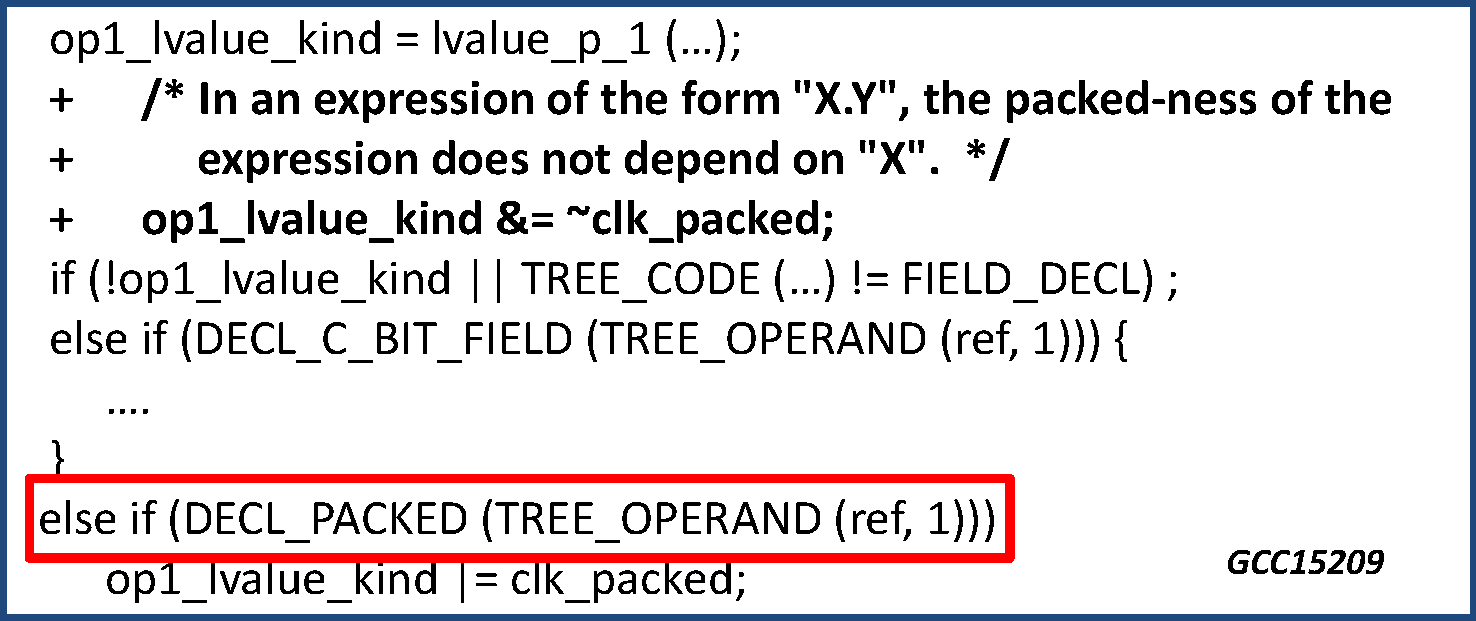
\includegraphics[width=3in]{figures/gcc15209}
\caption{A GCC Bug running out of memory}
\label{fig:GCC15209}
\end{center}
\end{figure}

GCC15209 shown in Figure~\ref{fig:GCC15209} in another example, where branch predicates are also useful. 
When reporting GCC15209, the user provides two similar inputs, one will run out of memory, and the other will not. During failure runs, the buggy branch highlighted in Figure~\ref{fig:GCC15209} will be taken, 
and during successful runs, that branch will not be taken. 
We can see that the buggy branch is very close to where the final patch is applied (8 lines omitting comments). 



\begin{figure}[t!]
\begin{center}
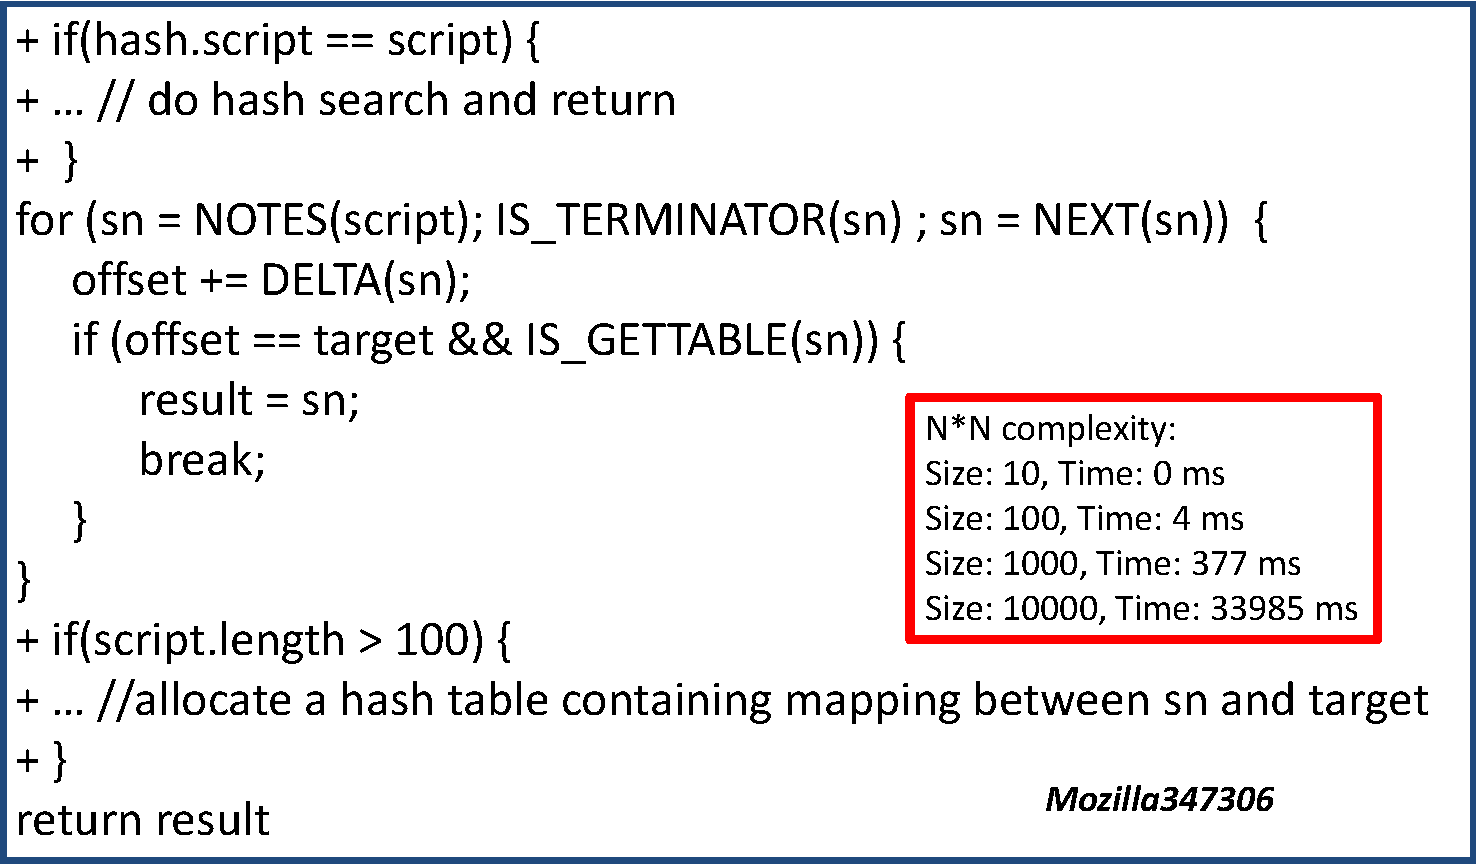
\includegraphics[width=3in]{figures/Mozilla347306}
\caption{A Mozilla Bug Containing $O(n^2)$ Complexity}
\label{fig:Mozilla347306}
\end{center}
\end{figure}

{\bf Mozilla347306} is caused by $O(n^2)$ complexity inside the buggy loop shown in Figure~\ref{fig:Mozilla347306}. 
The buggy loop is to search a related $sn$ for a given $target$ from data structure $script$. 
For one instance of the buggy loop, the search complexity is $O(n)$, and the number of instances for the buggy loop is also $O(n)$. 
This is how $O(n^2)$ complexity comes from. 
The fix is to use a hash table to contain the map between $sn$ and $target$ and change the search complexity from $O(n)$ to $O(1)$, when the length of script is longer than $100$.  
When reporting this bug, the user compared execution time under different input sizes to expose the $(n^2)$ complexity. 
If we can identify the buggy loop to developers, it would help them to diagnose and fix this bug. 


The above two examples help us answer questions asked earlier:

(1) Users tend to use comparison-based methods to notice performance loss, 
and they also use comparison-based methods to describe the abnormal performance. 
For MySQL44723, the end user compares inserting the same amount of data with different rows per insert,  
which he thinks should be finished in almost the same time. 
For Mozilla347306, the reporter compares similar inputs with different sizes to expose $O(n^2)$ complexity. 

(2) Users provide bad inputs and describe the abnormal performance 
when reporting performance bugs. For both of the above examples, 
users provide bad inputs they use and describe the abnormal performance they encounter. 
And for these two examples, the users also provide good inputs. 

(3) From these two examples, we can see that comparison between 
good and bad runs can provide useful diagnosis information. 
For MySQL44723, comparison can identify the branch leading to the fix. 
For Mozilla347306, comparison can point out loops where the final patch is applied. 

Of course, it is premature to draw any conclusion based on two
bugs. Next, we will comprehensively study 65 performance bugs.

\begin{table*}[tb!]
\small
\centering
{
\begin{tabular}{l|l}
\hline
{\bf Comparison} & {\bf Example}\\
\hline 
\multirow{3}{0.8in}{Applications} & {\bf Mozilla515287:} ``When running several Gmail instances in open tabs on my laptop (OS X), the \\
& CPU utilization is 15-20\% even while just idling. This has been tested with a blank profile, and no \\
& extensions. On Safari, the same open windows are at ~1.5\% CPU utilization."\\
\hline
\multirow{3}{0.8in}{Versions} & {\bf GCC12322:} ``The GCC-3.4 development snapshots take 5x or 6x as long to compile the \\
& computed-goto heavy core\_ops\_cg.c in Parrot. GCC-3.3 compiles this file in about five or six \\
& minutes on my slow  machine - GCC-3.4 takes 30 or more minutes."\\
\hline
\multirow{2}{0.8in}{Environments} & {\bf MySQL48429:} ``The performance of some sql with `group by' on partitioned table is very bad.''\\
&The user provides the execution time for same queries on partitioned table and unpartitioned table. \\
\hline
\multirow{2}{0.8in}{Sizes} & {\bf Mozilla104328:} ``On my windows machine my accumulated ~250 bookmarks takes about 2.5\% of  \\
&my normal 6 second startup. With a 1111 bookmark file my startup takes 42 seconds."\\
\hline
\multirow{2}{0.8in}{Similar Inputs} & {\bf Mozilla336944:} ``Happens on https://bugzilla.mozilla.org/ ... hogging the CPU the whole time\\
& (2-3 minutes or more instead of ~30 seconds for http://tinyurl.com/msj4y).'' \\
\hline
\end{tabular}
%\caption{Examples for Different Types of Comparison(this table needs to be changed)}
\caption{Examples of different types of comparison}
\label{tab:example}
}
\end{table*}


